\documentclass[USenglish]{article}

\usepackage{comment}
\newcommand{\lop}[0]{\mathcal{L}}
\newcommand{\lopd}[0]{\mathcal{L}_\Delta}
\newcommand{\lopdt}[0]{\mathcal{L}_{\Delta}}
\newcommand{\usol}[0]{\underline{\uvec{u}}_\Delta}
\newcommand{\usoldt}[0]{\underline{\uvec{u}}_\Delta}


\newcommand{\up}[0]{\underline{\uvec{u}}^{(p)}}

\newcommand{\usoldto}[0]{\tilde{\underline{\uvec{u}}}_\Delta}

\newcommand{\uapp}[0]{\uvec{u}_h}
\newcommand{\wapp}[0]{w_h}

\newcommand{\massmatrix}[0]{\mathcal{M}}

\newcommand{\tess}[0]{\mathcal{T}_h}


\newcommand{\uvec}[2][3]{\boldsymbol{#2\mkern-#1mu}\mkern#1mu}


\newcommand{\res}[0]{\textbf{R}}

\newcommand{\flux}[0]{\boldsymbol{F}}
\newcommand{\source}[0]{\boldsymbol{S}}
\newcommand{\ST}[0]{\boldsymbol{ST}_i^K}
\newcommand{\extra}[0]{\boldsymbol{ST}_i}


\newcommand{\elres}[0]{\uvec{\Phi}^K(\uapp)}
\newcommand{\noderes}[0]{\uvec{\Phi}^K_i(\uapp)}

\newcommand{\spacestuff}[0]{\bm{\phi}_i}

\newcommand{\cund}[0]{\underline{\uvec{c}}}

\newcommand{\lopdi}[0]{\mathcal{L}_{\Delta,i}}

\newcommand{\csoldt}[0]{\underline{\uvec{c}}_\Delta}

\newcommand{\basis}[0]{\uvec{v}}

\newcommand{\mis}[0]{\mu}
\newcommand{\red}[1]{{\color{red}#1 }}
\def\restriction#1#2{\mathchoice
              {\setbox1\hbox{${\displaystyle #1}_{\scriptstyle #2}$}
              \restrictionaux{#1}{#2}}
              {\setbox1\hbox{${\textstyle #1}_{\scriptstyle #2}$}
              \restrictionaux{#1}{#2}}
              {\setbox1\hbox{${\scriptstyle #1}_{\scriptscriptstyle #2}$}
              \restrictionaux{#1}{#2}}
              {\setbox1\hbox{${\scriptscriptstyle #1}_{\scriptscriptstyle #2}$}
              \restrictionaux{#1}{#2}}}
\def\restrictionaux#1#2{{#1\,\smash{\vrule height .8\ht1 depth .85\dp1}}_{\,#2}} 

\newcommand\swapifbranches[3]{#1{#3}{#2}}


\newcommand{\dt}{\Delta t}


\newcommand{\redun}[1]{{\color{red} {\large \textit{Is the following redundant?}} #1}}
\newcommand{\davide}[1]{{\color{blue}Davide: #1}}
\newcommand{\question}[1]{{\color{red} \large Question: #1 }}
\newcommand{\bbu}{\underline{\uvec{u}}}
\newcommand{\bbU}{\underline{\uvec{U}}}
\newcommand{\bbr}{\underline{\uvec{r}}}
\newcommand{\by}{\uvec{y}}
\newcommand{\bby}{\underline{\uvec{y}}}
\newcommand{\bG}{{\uvec{G}}}
\newcommand{\bbt}{\underline{t}}
\newcommand{\vecz}{\underline{0}}
\newcommand{\matz}{\underline{\underline{0}}}
\newcommand{\vecbeta}{\underline{\beta}}
\newcommand{\CIP}{\text{CIP}}
\newcommand{\OSS}{\text{OSS}}
\newcommand{\CFL}{\text{CFL}}



\newcommand{\undu}{\underline{\uvec{u}}}
\newcommand{\undy}{\underline{\uvec{y}}}
\newcommand{\undspacetilde}{\widetilde{\underline{\uvec{\phi}}}}
\newcommand{\undv}{\underline{\uvec{v}}}
\newcommand{\undw}{\underline{\uvec{w}}}
\newcommand{\undr}{\underline{\uvec{r}}}
\newcommand{\undz}{\underline{\uvec{z}}}
\newcommand{\lopdtp}[0]{\mathcal{L}_{\Delta,p}}
\newcommand{\usolp}[0]{\underline{\uvec{u}}_{\Delta}^{(p)}}
\newcommand{\Xp}[0]{X^{(p)}}
\newcommand{\Yp}[0]{Y^{(p)}}
\newcommand{\uex}[0]{\underline{\uvec{u}}_{ex}}
\newcommand{\uexp}[0]{\underline{\uvec{u}}_{ex}^{(p)}}
\newcommand{\lopdLp}[0]{\mathcal{L}_\Delta^{1,(p)}}
\newcommand{\lopdHp}[0]{\mathcal{L}_\Delta^{2,(p)}}
\newcommand{\embep}[0]{\mathcal{E}^{(p)}}
\newcommand{\projp}[0]{\Pi^{(p)}}
\newcommand{\trialspace}[1]{\varphi_{#1}} 
\newcommand{\trialspaceiter}[2]{\varphi_{#1}^{#2}} 
\newcommand{\trialtime}[1]{\psi^{#1}} 
\newcommand{\trialtimeiter}[2]{\psi^{#1,#2}} 
\newcommand{\trialspacetime}[1]{\vartheta^{#1}} 
\newcommand{\trialspacetimeiter}[2]{\vartheta^{#1,#2}}

\newcommand{\trialspaceFVp}[1]{\varphi_{#1}} 
\newcommand{\trialspaceFVc}[1]{\lambda_{#1}} 
\newcommand{\APNPM}{{ADER-$\mathbb P_N \mathbb P_M$ }}

\newcommand{\undG}[0]{\underline{\uvec{G}}}

\newcommand{\lore}[1]{{\large \textcolor{magenta}{Lore: #1}}} 
\newcommand{\hpsi}{\widehat{\psi}}
\newcommand{\hphi}{\widehat{\phi}}
\newcommand{\uhphi}{\underline{\widehat{\phi}}}


\newcommand{\ADERIWF}{ADER-IWF}
\newcommand{\ADERRK}{ADER-IWF-RK} 

\newcommand{\Bp}{\mathcal{B}} 
\newcommand{\Cp}{\mathcal{C}} 
\newcommand{\Dp}{\mathcal{D}} 

\newcommand{\IM}{\mathcal{H}} 
\newcommand{\co}{u} 
\newcommand{\va}{v} 

\newcommand{\SRK}{S} 

\newcommand{\ADERdu}{ADERdu}
\newcommand{\ADERu}{ADERu} 
\newcommand{\cADER}{cADER} 

\newcommand{\CC}{C5}

\usepackage{fullpage}
\usepackage{amsmath,amsfonts,amsthm,amssymb}
\usepackage{color}
\usepackage[dvipsnames]{xcolor}
\usepackage{ifpdf}
\usepackage{psfrag}
\usepackage{graphicx,graphics}
\usepackage{hhtensor}
\usepackage{comment}
\usepackage[small]{caption}
\usepackage{subcaption}
\usepackage{tabularx}

\usepackage{xparse}
\usepackage{bigints}

\usepackage{url}
\usepackage{hyperref}
\usepackage{todonotes}
\usepackage{cleveref}
\usepackage{ulem} \normalem
% ------------------------------------------
\newtheorem{theorem}{Theorem}[section]
\newtheorem{corollary}[theorem]{Corollary}
\newtheorem{lemma}[theorem]{Lemma}
\newtheorem{proposition}[theorem]{Proposition}
\newtheorem{prop}[theorem]{Proposition}
\newtheorem{remark}[theorem]{Remark}
\newtheorem{definition}[theorem]{Definition}
\newtheorem{example}[theorem]{Example}
\newtheorem{assumption}[theorem]{Assumption}
\newtheorem{conclusion}[theorem]{Conclusion}

\usepackage{cancel}
\usepackage{algorithm,algorithmic}
\usepackage{enumitem}

\usepackage{pgfplots}
\usepackage{pgfplotstable}
\usepackage{tikz}

\usetikzlibrary{fillbetween}
\usepgfplotslibrary{fillbetween}

\usetikzlibrary{shapes.misc}
\usetikzlibrary{math} 

\usetikzlibrary{arrows}

%\usetikzlibrary{external}
%\tikzexternalize[prefix=figures/]

\graphicspath{../Stochastic_results}

\newcommand{\R}{\mathbb R}
\newcommand{\Z}{\mathbb Z}
\newcommand{\N}{\mathbb N}
\newcommand{\C}{\mathbb C}
\newcommand{\Q}{\mathbb Q}
\newcommand{\K}{\mathbb K}
\renewcommand{\L}{\mathcal L}
\newcommand{\I}{\mathcal I}
\newcommand{\PP}{\mathbb P}
\newcommand{\TT}{\mathcal{T}}
\newcommand{\normal}{\mathbf{N}}

\renewcommand{\SS}{\mathcal{S}}
\newcommand{\KK}{\mathcal{K}}
\newcommand{\EE}{\mathcal{E}}

% ---- Notation Philipp
\newcommand{\ww}[1]{\underline{#1}}
\renewcommand{\div}{\operatorname{div}}
\newcommand{\est}[1]{\left\langle#1\right\rangle}
\newcommand{\bU}{\mathbf{U}}
\newcommand{\bH}{\mathbf{H}}
\newcommand{\dd}{\mathrm{d}}
\newcommand{\bV}{\mathbf{V}}
\newcommand{\mean}[1]{\overline{#1}}
\newcommand{\bbfh}{{\mathbf {f}^h}}
\newcommand{\Ol}{\mathcal{O}}
\newcommand{\WW}{\mathrm{W}}
\newcommand{\LL}{\mathcal{L}}
\newcommand{\II}{\hat{I}_0}
\newcommand{\1}{\begin{pmatrix}
		1\\
		1
\end{pmatrix}}


\newcommand\norm[1]{\left\lVert#1\right\rVert}

\newcommand{\tp}{t^{n+1}}
\newcommand{\tn}{t^{n}}


\renewcommand{\vec}[1]{\ww{#1}}
\NewDocumentCommand{\mat}{mo}{%
	\IfValueTF{#2}{%
		\underline{\underline{#1}}{#2}
	}{%
		\underline{\underline{#1}}\,
	}%
}
%Davide

\usepackage{bbm}
\def\bbc{\underline{\boldsymbol{\alpha}}}
\def\bc{\boldsymbol{\alpha}}
\def\bbu{\underline{\boldsymbol{u}}}
\def\bu{\boldsymbol{u}}
\def\br{\boldsymbol{r}}
\def\bd{\mathbf{d}}
\def\bbd{\underline{\mathbf{d}}}
\def\bphi{\underline{\phi}}
\def\M{\underline{\underline{\mathrm{M}}}}
\def\S{\underline{\underline{\mathrm{S}}}}
\def\ADERClassical{cADER}
\def\addref{{\color{red}\Large ADD REFERENCEs!}}

%Colors 
\definecolor{darkspringgreen}{rgb}{0., 0.55, 0.3}
\definecolor{dartmouthgreen}{rgb}{0.05, 0.5, 0.06}
\definecolor{etonblue}{rgb}{0.59, 0.78, 0.64}
\definecolor{airforceblue}{rgb}{0., 0.4, 0.66}
\definecolor{arylideyellow}{rgb}{0.91, 0.84, 0.42}
\definecolor{emerald}{rgb}{0.31, 0.78, 0.47}
\definecolor{uclagold}{rgb}{1.0, 0.7, 0.0}
\definecolor{cadmiumorange}{rgb}{0.93, 0.53, 0.18}


\newcommand{\maria}[1]{{\color{red} maria: #1}}
\definecolor{burg}{rgb}{0.5, 0.0, 0.13}
\newcommand{\delete}[1]{{\color{burg} delete: #1}}

\begin{document}
	\title{ConvAE tests} 

\begin{enumerate}
	\item Model1
	\begin{itemize}
		\item Conv Layers (ch in, ch out, kernel, stride, padding =0 )
		\begin{itemize}
			\item (  1,   4, 2, 1, 0)
			\item (  4,  16, 2, 1, 0)
			\item ( 16,  32, 4, 2, 0)
			\item ( 32,  64, 4, 2, 0)
			\item ( 64, 128, 4, 2, 0)
			\item (128, 128, 4, 2, 0)
			\item (128, 128, 4, 2, 0)
			\item (128, 128, 4, 2, 0)
		\end{itemize}
		\item Dense layer: 512=2*2*128 -> n\_latent
		\item Sizes at layers: 256,255,254,126,62,30,14,6,2
	\end{itemize}
	\item Model2
	\begin{itemize}
		\item Conv Layers (ch in, ch out, kernel, stride, padding =0 )
		\begin{itemize}
			\item (  1,   4, 2, 1, 0)
			\item (  4,  16, 2, 1, 0)
			\item ( 16,  32, 4, 2, 0)
			\item ( 32,  64, 4, 2, 0)
			\item ( 64, 128, 4, 2, 0)
			\item (128, 128, 4, 2, 0)
			\item (128, 128, 4, 2, 0)
		\end{itemize}
		\item Dense layer: 4608 = 6*6*128 -> n\_latent
		\item Sizes at layers: 256,255,254,126,62,30,14,6
	\end{itemize}
	
\end{enumerate}

\begin{figure}
	
	\newcommand{\method}{POD}
	\newcommand{\methodlabel}{POD}
	
	\begin{tikzpicture}
		\begin{axis}[
			ymode=log,
			ylabel = Error,
			ymin=1.e-3,ymax=1.e-2,
			grid=major,
			legend pos= north east,
			legend style={nodes={scale=0.6, transform shape}},
			width=.48\textwidth
			]
			\addplot[blue, mark color=none, only marks,mark=square] table [x=Param, y=error]{errors_param_trial_001_batch_004_n_dense_006.txt};
			\addlegendentry{M1 batch4 n6}
			\addplot[red, mark color=none, only marks,mark=triangle] table [x=Param, y=error]{errors_param_trial_001_batch_004_n_dense_014.txt};
			\addlegendentry{M1 batch4 n14}
			\addplot[black, mark color=none, only marks, mark=o] table [x=Param, y=error]{errors_param_trial_001_batch_004_n_dense_030.txt};
			\addlegendentry{M1 batch4 n30}
%			\addplot[red, dashed] table [x=params_training, y=\method_6,  col sep=comma]{\testname/training_errors.csv};
%			\addlegendentry{\methodlabel 6}
%			\addplot[blue, dashdotted] table [x=params_training, y=\method_14,  col sep=comma]{\testname/training_errors.csv};
%			\addlegendentry{\methodlabel 14}
		\end{axis}
	\end{tikzpicture}
	\begin{tikzpicture}
			\begin{axis}[
		ymode=log,
%		ylabel = Error,
		ymin=1.e-3,ymax=1.e-2,
		grid=major,
		legend pos= north east,
		legend style={nodes={scale=0.6, transform shape}},
		width=.48\textwidth
		]
		\addplot[blue, mark color=none, only marks,mark=square] table [x=Param, y=error]{errors_param_trial_001_batch_016_n_dense_006.txt};
		\addlegendentry{M1 batch16 n6}
		\addplot[red, mark color=none, only marks,mark=triangle] table [x=Param, y=error]{errors_param_trial_001_batch_016_n_dense_014.txt};
		\addlegendentry{M1 batch16 n14}
		\addplot[black, mark color=none, only marks, mark=o] table [x=Param, y=error]{errors_param_trial_001_batch_016_n_dense_030.txt};
		\addlegendentry{M1 batch16 n30}
		%			\addplot[red, dashed] table [x=params_training, y=\method_6,  col sep=comma]{\testname/training_errors.csv};
		%			\addlegendentry{\methodlabel 6}
		%			\addplot[blue, dashdotted] table [x=params_training, y=\method_14,  col sep=comma]{\testname/training_errors.csv};
		%			\addlegendentry{\methodlabel 14}
	\end{axis}
	\end{tikzpicture}
	\begin{tikzpicture}
	\begin{axis}[
		ymode=log,
		ylabel = Error,
		ymin=1.e-3,ymax=1.e-2,
		grid=major,
		legend pos= north east,
		legend style={nodes={scale=0.6, transform shape}},
		width=.48\textwidth
		]
		\addplot[blue, mark color=none, only marks,mark=square] table [x=Param, y=error]{errors_param_trial_001_batch_180_n_dense_006.txt};
		\addlegendentry{M1 batch180 n6}
		\addplot[red, mark color=none, only marks,mark=triangle] table [x=Param, y=error]{errors_param_trial_001_batch_180_n_dense_014.txt};
		\addlegendentry{M1 batch180 n14}
		\addplot[black, mark color=none, only marks, mark=o] table [x=Param, y=error]{errors_param_trial_001_batch_180_n_dense_030.txt};
		\addlegendentry{M1 batch180 n30}
		%			\addplot[red, dashed] table [x=params_training, y=\method_6,  col sep=comma]{\testname/training_errors.csv};
		%			\addlegendentry{\methodlabel 6}
		%			\addplot[blue, dashdotted] table [x=params_training, y=\method_14,  col sep=comma]{\testname/training_errors.csv};
		%			\addlegendentry{\methodlabel 14}
	\end{axis}
\end{tikzpicture}
\hfill
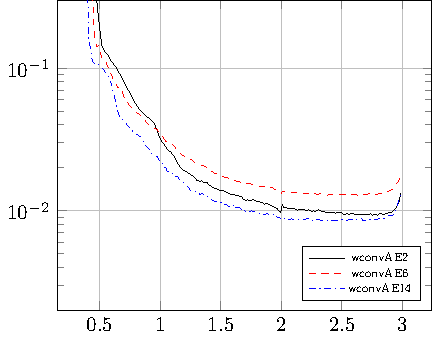
\includegraphics[width=0.45\textwidth]{training_errors-figure5.pdf}
%\begin{tikzpicture}
%	\begin{axis}[
%		ymode=log,
%		%		ylabel = Error,
%		ymin=1.e-3,ymax=1.e-2,
%		grid=major,
%		legend pos= north east,
%		legend style={nodes={scale=0.6, transform shape}},
%		width=.48\textwidth
%		]
%		\addplot[blue, mark color=none, only marks,mark=square] table [x=Param, y=error]{errors_param_trial_002_batch_004.txt};
%		\addlegendentry{M1 batch4 n10}
%		\addplot[red, mark color=none, only marks,mark=triangle] table [x=Param, y=error]{errors_param_trial_002_batch_016.txt};
%		\addlegendentry{M1 batch16 n10}
%		\addplot[black, mark color=none, only marks, mark=o] table [x=Param, y=error]{errors_param_trial_002_batch_180.txt};
%		\addlegendentry{M1 batch180 n10}
%		%			\addplot[red, dashed] table [x=params_training, y=\method_6,  col sep=comma]{\testname/training_errors.csv};
%		%			\addlegendentry{\methodlabel 6}
%		%			\addplot[blue, dashdotted] table [x=params_training, y=\method_14,  col sep=comma]{\testname/training_errors.csv};
%		%			\addlegendentry{\methodlabel 14}
%	\end{axis}
%\end{tikzpicture}

	
	\caption{ConvAE errors with different models (bottom right is the old one)}
\end{figure}

\end{document}
